\cleardoublepage
\chapter{Software}\label{chap:software}
% To do: 
% Color Scheme
% Red - Not started
% Yellow - In progress
% Blue - Done, under approval
% Green - Done and approved
\todo[inline,color=blue!40]{closed - v1.1 finished 16/07/2021, to review}
%\todo[inline,color=blue!40]{*Chapter Introduction}
%\todo[inline,color=blue!40]{*1 - Microphone}
%\todo[inline,color=blue!40]{*2 - Microcontroller}
%\todo[inline,color=blue!40]{ a) Peripherals}
%\todo[inline,color=blue!40]{ b) FFT implementation}
%\todo[inline,color=blue!40]{ c) Fixed-Point Square Root}
%\todo[inline,color=blue!40]{*3 - MatLab}
%\todo[inline,color=blue!40]{*4 - Level Identification}
%%%%%%%%%%%%%%%%%%%%%%%%%%%%%%%%%% Writing %%%%%%%%%%%%%%%%%%%%%%%%%%%%%%%%%%%
This chapter is dedicated to presenting every piece of software necessary, for the interaction between all the elements that are part of the setup used in all the stages until the implementation, with a brief explanation of how they work and what is their purpose in the setup. All the elements are not necessarily used at the same time in the setup and how they will interact with each other will be presented in chapter~\ref{chap:Tests}.
\section{Microphone}
As the first measurements will be taken recurring to a microphone, it requires a different approach to the type of interaction when compared to the future application, where a different sensor is used to detect the vibration. To obtain access and record the information from the microphone and for this case in specific, since it is being used the microphone from a phone, will require different pieces of software to use in the phone side and the \acrshort{pc}, to allow the access to the second to the microphone of the first. Also, on the \acrshort{pc} side it is necessary to record the information from the microphone and store it as desired.

The two components for this purpose will be the use of the WOMic software as the bridge between the phone and the computer, and \acrshort{matlab} to record the information from the microphone. The second software can also be used to later process the recorded data, helping the understanding of the obtained information. 
\subsection*{WOMic}
The use of the application and the microphone of the phone is simple, although the installation and the configuration requires some time. For that, it is required to install the software \textit{WOMic} in both devices, this allows the use of the microphone of the phone in real-time. In the phone the software is available for Android and IOS and is responsible to transmit what is captured from the microphone, in the computer the client application and a virtual device must be installed to use the microphone in the \acrshort{pc} to perform any type of tasks, this connection can be made over \acrshort{usb}, Bluetooth, \acrshort{wifi} and \acrshort{wifi} Direct.

In order to save what is captured from the microphone, the software is split in three main block with different purposes, the \textit{WOMic App} runs in the phone, samples the input of the microphone and transmit it to the computer, the \textit{WOMic Client}, runs in the \acrshort{pc}, connect to the app in the phone, and receive the data from the microphone, which is transmitted to the \textit{WOMic Virtual Device} on which a real microphone device is simulated and provides the audio to any application or program in the \acrshort{pc}, as illustrated in figure~\ref{fig:diagramWOMIC}.

\begin{figure}[]
    \centering
    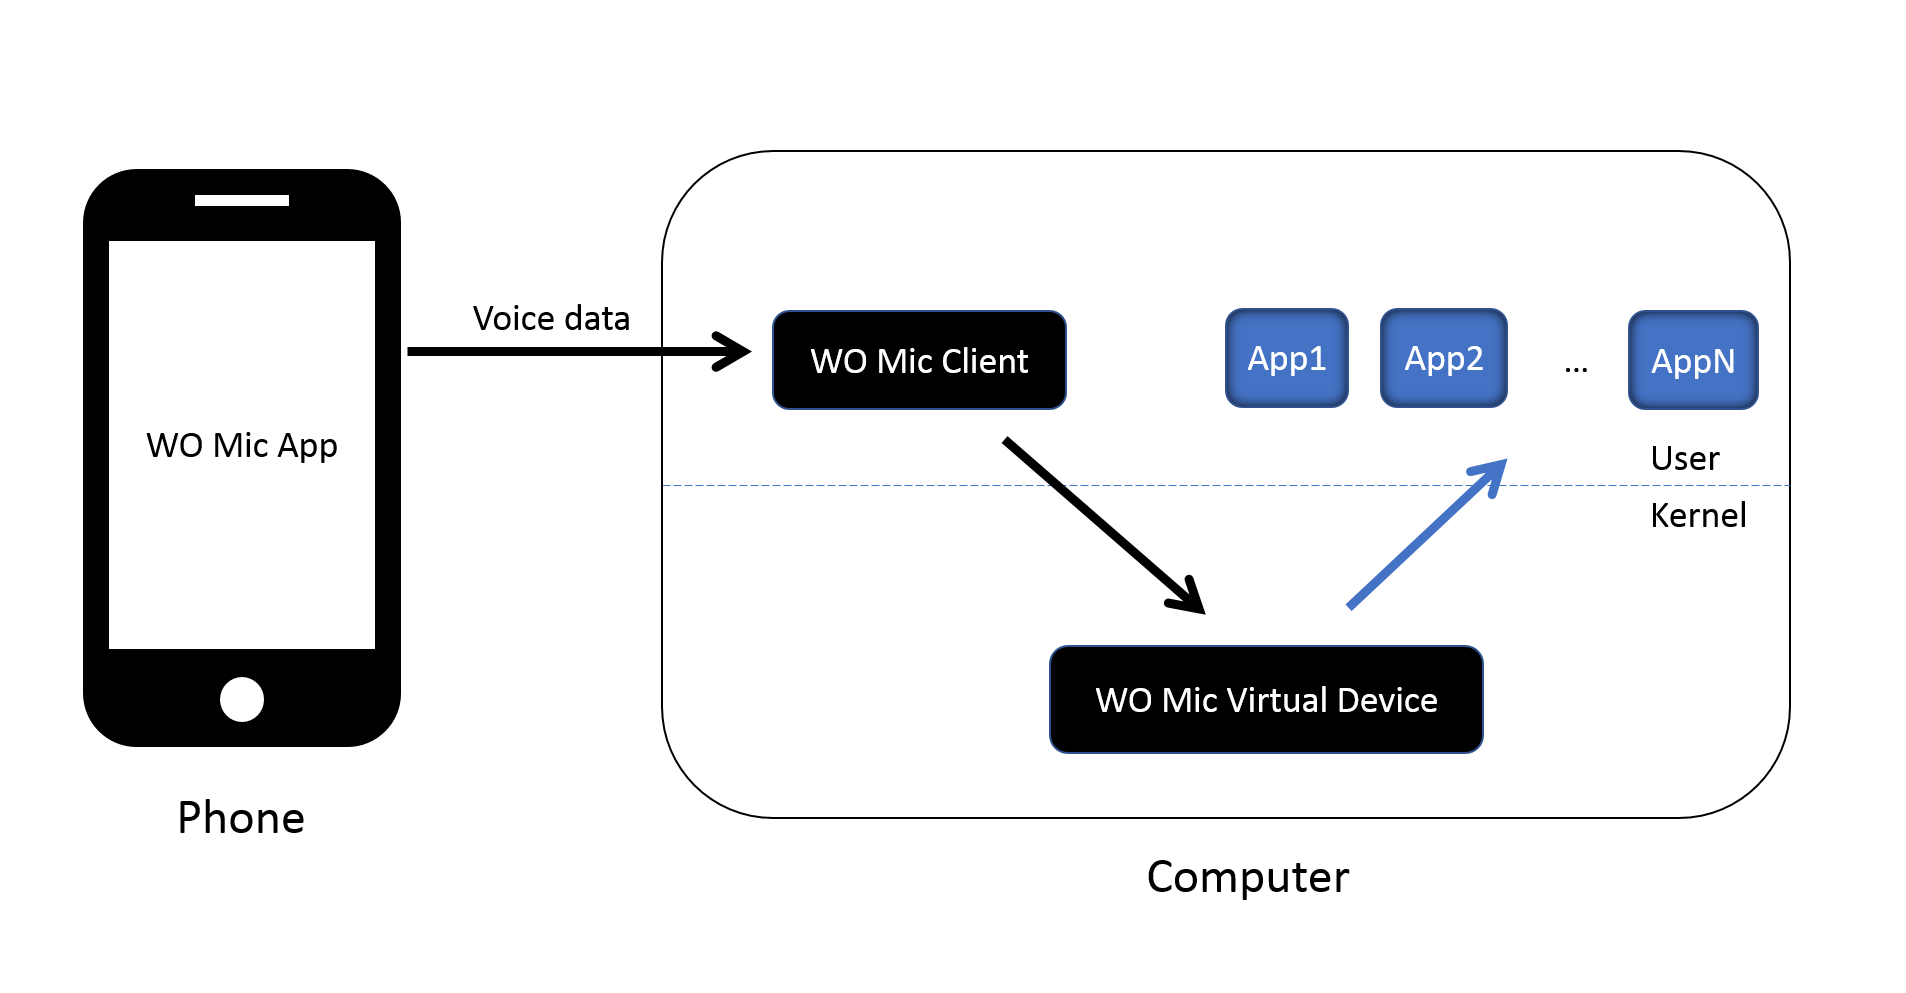
\includegraphics[width=0.65\textwidth]{Chapters/5CHP/Images/WOMICDiag.png}
    \caption{Flow of data in the components of the software}{\cite{WOMicFREE}}
    \label{fig:diagramWOMIC}
\end{figure}
In addition to this, it is also necessary to install the drivers of the phone in use, if the connection is made over USB. To allow the access of the microphone in the \acrshort{pc}, the transport mode must be selected on the phone application, USB in this case, in the app settings and after that start the application. In the PC the client software must be initialized and connected to the phone in the following order \textit{$>$Connection$>$Connect...} a new window will open, on which the USB must be selected as transport type and finalizing by pressing \textit{Connect}. With this, the microphone of the phone is available for use in the \acrshort{pc}\cite{WOMicFREE}.
\section{Microcontroller}

To capture the signal obtained from the sensor, for a later processing and analysis, is necessary to develop some specific pieces of software. Some are related to the microcontroller itself, needed to interact with the sensors, actuators and to communicate with the \acrshort{pc}, beside that some algorithms were used to process the data that are relevant for the application. A brief explanation of each piece of software used is explained, with some details of their functioning and their purpose.
\subsection{Peripherals}
\subsubsection*{Timers}
In the configuration, two different timers were set, with the same configuration, one is used to measure the execution time of the algorithm and the other is used to set the amount of time that the pin that triggers the solenoid is high. In this case were used Timer0\_A3 and Timer1\_A3, in both the counter mode of the timer is up, the division factor of the clock is 1 and they were set with a CCRx equal to 499, with this a interruption will occur at every 500$\mu$s.
\subsubsection*{ADC}
The LaunchPad in use offers \acrshort{adc} with a 10-bit, from the available pins, analog input 2 is selected. This input should be configured with the desire setting, to start is mandatory to disable the digital port of the pin to eliminate the flow of parasitic current flow, with the PySELx bits, by setting these bits HIGH it automatically enables the analog function of the port, although is still necessary to select the channel to conversion. The \acrshort{adc} will function in the sample and hold mode, using the timer from the \acrshort{adc} as the source of the sampling signal, the sample and hold period can be changed by software, to define the amount of clock cycles between each sample. 
\subsubsection*{eUSCI}
The \acrshort{eusci} is used in \acrshort{uart} mode to transfer data between the microcontroller and the \acrshort{pc}, is used during the tests phase to perform two types of tests, one to test the algorithm and the other to receive data and send it to the \acrshort{pc}. Both \acrshort{eusci}\_A0 and \acrshort{eusci}\_A1 support \acrshort{uart} mode, unlike the \acrshort{eusci}\_B0, the selected was the first, since works over the \acrshort{usb} connection. In Transmission and Receiving, they were both set to work by polling with 115200bps of baud-rate, 8-bit, \acrshort{lsb} first, no parity, no address and 1 stop bit.
\subsection{FFT implementation}\label{subsec:fftImp}
To process the signal captured from the \acrshort{adc}, a \acrshort{fft} algorithm is used. Two algorithms were considered to be used in the microcontroller, a Fixed-Point and a Floating-Point versions, this algorithm was discovered by Cooley and Tukey in the beginning of the computer revolution and based on the complex \acrshort{dft}. The implementations used are based in \acrshort{fft} algorithm, and analyzing the Fixed-Point and the Floating-Point implementations side by side, they are quite similar, the main difference is in the data types used in each of the implementations, the fixed point can be adapted for the different types of signed integers, from 8-bits to 64-bits and uses a look-up table with the correspondent values of Sine and Cosine, used to calculate the real and imaginary in the frequency domain. This saves processing time, since isn't necessary to calculate these values, while the algorithm is running, on the other hand this limits the size of the vector to be processed, to be in maximum the size of the look-up table, unless the implementation is adapted. This implementation is less time consuming for the microcontroller. The Floating-Point version calculates the values of the Sine and Cosine, while processing the data. Since it deals with values like float or double, will require more memory and computational resources from the microcontroller, if the same is used in both cases. Both implementation can be found on a repository in~\cite{262588213843476FixFft,Dannyf00FloatingPointFFTBenchmarka}, for a implementation from scratch there is also possible to find pseudo-code for that~\cite{smith1997scientist}.

The algorithms in use were adapted to fit in the purpose of the implementation for the microcontroller in use, as well as removed some options like the \acrshort{ifft}, which won't be necessary to use in this application.

After performing the \acrshort{fft} algorithm in the input data vector, is necessary to calculate the magnitude of the resulting data, since the algorithm returns complex values. To obtain the magnitude of the data in frequency is a simple mathematical operation and is described in~\ref{eq:magnitude}.
\begin{equation}\label{eq:magnitude}
    M = \sqrt{Re^2 + Im^2}
\end{equation}
\subsection{Fixed-Point Square Root}
For the application where the Fixed-Point is used it is convenient to only deal with integers, after performing the \acrshort{fft} is necessary to calculate the magnitude of the signal, relative to the frequency, since the data returned from the algorithm is complex. For that as known, is necessary to use a the square root, several implementation of a Fixed-Point square root can be found, the implementation in use is an adaptation of the integer-to-integer version, from the repository~\cite{ChmikeFpsqrta}, in the used square root function, the input argument is a 32-bit value and the output a 16-bit value.

\section{MatLab}
This computational platform has various resources, with a lot of appliances. For the purpose of the developed work only a few simple functions of this platform. In a initial stage, is going to be taken advantages of some of their function to generate random signals, in order to test the viability and precision of the \acrshort{fft} algorithm that will be used in a microcontroller environment, this requires the use of some basic mathematical functions and the serial-port, the first is used to generate the random signal and the secondo to send the signal to to the microcontroller via \acrshort{uart}, so it can be processed and the resulting data can be compared with the original.

On other sets of tests functions to record data from a certain audio input were used, to record the input of the microphone, each time that the \acrshort{lpg} bottle is hit with the hammer. Beside this, the \acrshort{fft} function from the MATLAB is used to verify the response in frequency of the hit.

Before the final application, is also need to verify the type of signals obtain in the sensors, after captured in the microcontroller the raw data is sent via \acrshort{uart} to, once again, process them in the \acrshort{fft} function of \acrshort{matlab}. 
\section{Level Identification}
In chapter~\ref{chap:stArt}, we have seen that, when stimulated with a hammer, the frequency peak increases if the liquid level inside the \acrshort{lpg} bottle decreases. If the conditions of the stimulation and measurement are consistent every time that they are performed, the results should be consistent for each liquid level. Considering this, it should be quite easy to develop a simple algorithm to identify the liquid level, basically the only thing necessary is to identify a frequency interval, where the peaks are, to reduce the searching time. As we will see it is not as simple as imagined, to determine the liquid level will be considered other factors like, the first peaks, the energy around the peaks and the one with the highest energy. In a first stage, before defining a frequency interval, all the spectrum must be considered, not only in the data captured by the sensors, but as well in the microphone.

Based on these notes, only after observing several samples of measured signals is it possible to properly define what is the interval and how to conjugate the characteristics of the spectrum, to define the algorithm to identify the liquid level. 
\section{End of chapter considerations}
The current chapter was used to present the software elements that will be used. Part of the presented ones, are not directly part of the processing/identification process, but are essential for the function of the software. This is the reason why they are mentioned and the important details from them are mentioned.

Combining these elements with the physical elements, mentioned in the previous chapter, we are now able to move to the final step, where we will be able to perform the necessary tests to evaluate the viability of each element of the defined architecture for the system. This will be done in the following chapter.
%\addcontentsline{toc}{section}{References}
